\documentclass{article}

\usepackage{amsmath,amssymb}
\usepackage{tikz}
\usepackage{pgfplots}
\usepackage{xcolor}
\usepackage[left=2.1cm,right=3.1cm,bottom=3cm,footskip=0.75cm,headsep=0.5cm]{geometry}
\usepackage{enumerate}
\usepackage{enumitem}
\usepackage{marvosym}
\usepackage{tabularx}

\usepackage{listings}
\definecolor{lightlightgray}{rgb}{0.95,0.95,0.95}
\definecolor{lila}{rgb}{0.8,0,0.8}
\definecolor{mygray}{rgb}{0.5,0.5,0.5}
\definecolor{mygreen}{rgb}{0,0.8,0.26}
\lstdefinestyle{java} {language=java}
\lstset{language=java,
	basicstyle=\ttfamily,
	keywordstyle=\color{lila},
	commentstyle=\color{lightgray},
	stringstyle=\color{mygreen}\ttfamily,
	backgroundcolor=\color{white},
	showstringspaces=false,
	numbers=left,
	numbersep=10pt,
	numberstyle=\color{mygray}\ttfamily,
	identifierstyle=\color{blue},
	xleftmargin=.1\textwidth, 
	%xrightmargin=.1\textwidth,
	escapechar=§,
}

\usepackage[utf8]{inputenc}

\renewcommand*{\arraystretch}{1.4}

\newcolumntype{L}[1]{>{\raggedright\arraybackslash}p{#1}}
\newcolumntype{R}[1]{>{\raggedleft\arraybackslash}p{#1}}
\newcolumntype{C}[1]{>{\centering\let\newline\\\arraybackslash\hspace{0pt}}m{#1}}

\newcommand{\E}{\mathbb{E}}
\DeclareMathOperator{\rk}{rk}
\DeclareMathOperator{\Var}{Var}
\DeclareMathOperator{\Cov}{Cov}

\title{\textbf{Rechnernetze, Übung 2}}
\author{\textsc{Henry Haustein}}
\date{}

\begin{document}
	\maketitle
	
	\section*{Aufgabe 1}
	\begin{enumerate}[label=(\alph*)]
		\item Es gilt
		\begin{align}
			b &< 2\cdot B\cdot \log_2(S) \notag \\
			B &> \frac{b}{2\cdot\log_2(S)} \notag \\
			&> \frac{9600\text{ Bit/s}}{2\cdot\log_2(16)} \notag \\
			&> 1200 \text{ Hz} \notag
		\end{align}
		Für die Symbolrate (= Baudrate $BR$) gilt
		\begin{align}
			b &= BR\cdot \log_2(S) \notag \\
			BR &= \frac{b}{\log_2(S)} \notag \\
			&= \frac{9600\text{ Bit/s}}{\log_2(16)} \notag \\
			&= 2400 \text{ Bd} \notag
		\end{align}
		Der Informationsgehalt jedes Symbols ist $\log_2(16)=4$ Bit.
		\item Der Signalrauschabstand $SNR$ ist $10^{\frac{SNR_{dB}}{10}} = 15.8489$. Es gilt
		\begin{align}
			b < B\cdot\log_2(1+SNR) \notag \\
			B &> \frac{b}{\log_2(1+SNR)} \notag \\
			&> \frac{9600 \text{ Bit/s}}{\log_2(1+2.2974)} \notag \\
			&> 2356.0696 \text{ Hz} \notag
		\end{align}
		\item Wieder ist der Signalrauschabstand $SNR$ $10^{\frac{SNR_{dB}}{10}} = 1000$. Damit gilt
		\begin{align}
			b < B\cdot\log_2(1+SNR) \notag \\
			B &> \frac{b}{\log_2(1+SNR)} \notag \\
			&> \frac{9600 \text{ Bit/s}}{\log_2(1+1000)} \notag \\
			&> 963.1566 \text{ Hz} \notag
		\end{align}
		Aber das Nyquist-Theorem gibt eine Mindestbandbreite von 1200 Hz vor, diese kann also nicht unterschritten werden.
	\end{enumerate}

	\section*{Aufgabe 2}
	\begin{enumerate}[label=(\alph*)]
		\item Bestimmen wir zuerst die Bandbreite, die wir durch diese Leitung bekommen. $S=2$, da es sich hier um ein digitales Signal, also nur um 1 oder 0 handelt.
		\begin{align}
			b &< 2\cdot B\cdot \log_2(S) \notag \\
			&< 2\cdot 60000\text{ Hz}\cdot \log_2(2) \notag \\
			&< 120000 \text{ Bit/s} \notag
		\end{align}
		Bei 1023 Quantisierungsintervallen gibt es 1024 Signalstufen und damit müssen bei jedem Abtasten $\log_2(1024)=10$ Bit Information durch die Leitung geschickt werden, um die richtige Signalstufe zu übermitteln. Die Leitung hat eine maximale Kapazität von 120000 Bit/s, es können also maximal 12000 Abtastvorgänge pro Sekunde geschehen, also $f_A=12000$ Hz. Nach dem Abtasttheorem von Shannon darf die Grenzfrequenz 6000 Hz nicht überschreiten. Es sind Qualitätseinbußen bei der Tonspur eines Videos zu erwarten, denn der für Menschen wahrnehmbare Frequenzbereich liegt im Bereich von 20 Hz bis 20 kHz, aber die Grenzfrequenz liegt bei nur 6 kHz!
		\item 1 Bit: extremes Rauschen, Knacken, Unterbrechungen; 4 Bit: starkes Rauschen; 8 Bit: leises Hintergrundrauschen; heute üblich: Codierung mit 16 Bit pro Sample; Musikproduktion: 32 Bit
	\end{enumerate}

	\section*{Aufgabe 3}
	\begin{enumerate}[label=(\alph*)]
		\item Amplitudentastung
		\begin{center}
			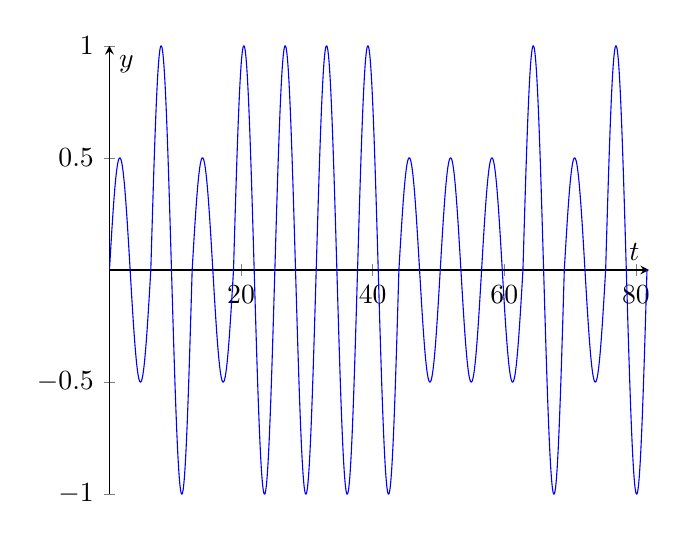
\begin{tikzpicture}
			\begin{axis}[
			xmin=0, xmax=82, xlabel=$t$,
			ymin=-1, ymax=1, ylabel=$y$,
			samples=400,
			axis x line=middle,
			axis y line=middle,
			domain=0:82,
			]
			\addplot[mark=none,smooth,blue,domain=0:2*pi] {0.5*sin(deg(x))};
			\addplot[mark=none,smooth,blue,domain=2*pi:4*pi] {sin(deg(x))};
			\addplot[mark=none,smooth,blue,domain=4*pi:6*pi] {0.5*sin(deg(x))};
			\addplot[mark=none,smooth,blue,domain=6*pi:8*pi] {sin(deg(x))};
			\addplot[mark=none,smooth,blue,domain=8*pi:10*pi] {sin(deg(x))};
			\addplot[mark=none,smooth,blue,domain=10*pi:12*pi] {sin(deg(x))};
			\addplot[mark=none,smooth,blue,domain=12*pi:14*pi] {sin(deg(x))};
			\addplot[mark=none,smooth,blue,domain=14*pi:16*pi] {0.5*sin(deg(x))};
			\addplot[mark=none,smooth,blue,domain=16*pi:18*pi] {0.5*sin(deg(x))};
			\addplot[mark=none,smooth,blue,domain=18*pi:20*pi] {0.5*sin(deg(x))};
			\addplot[mark=none,smooth,blue,domain=20*pi:22*pi] {sin(deg(x))};
			\addplot[mark=none,smooth,blue,domain=22*pi:24*pi] {0.5*sin(deg(x))};
			\addplot[mark=none,smooth,blue,domain=24*pi:26*pi] {sin(deg(x))};
			
			\end{axis}
			\end{tikzpicture}
		\end{center}
		Frequenztastung
		\begin{center}
			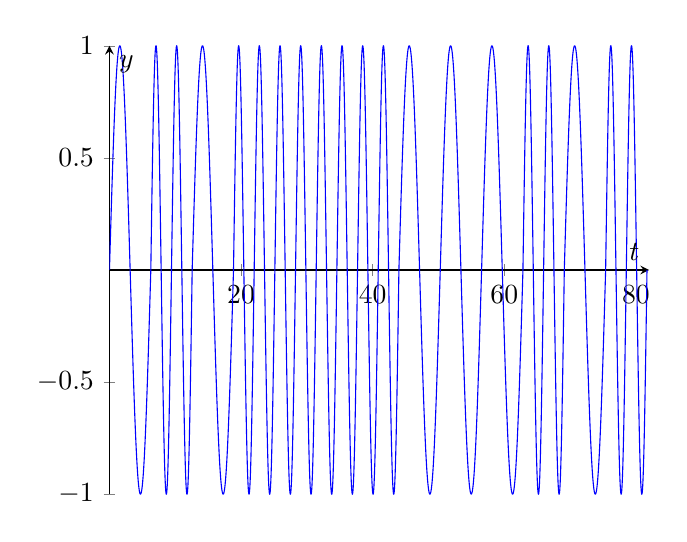
\begin{tikzpicture}
			\begin{axis}[
			xmin=0, xmax=82, xlabel=$t$,
			ymin=-1, ymax=1, ylabel=$y$,
			samples=400,
			axis x line=middle,
			axis y line=middle,
			domain=0:82,
			]
			\addplot[mark=none,smooth,blue,domain=0:2*pi] {sin(deg(x))};
			\addplot[mark=none,smooth,blue,domain=2*pi:4*pi] {sin(deg(2*x))};
			\addplot[mark=none,smooth,blue,domain=4*pi:6*pi] {sin(deg(x))};
			\addplot[mark=none,smooth,blue,domain=6*pi:8*pi] {sin(deg(2*x))};
			\addplot[mark=none,smooth,blue,domain=8*pi:10*pi] {sin(deg(2*x))};
			\addplot[mark=none,smooth,blue,domain=10*pi:12*pi] {sin(deg(2*x))};
			\addplot[mark=none,smooth,blue,domain=12*pi:14*pi] {sin(deg(2*x))};
			\addplot[mark=none,smooth,blue,domain=14*pi:16*pi] {sin(deg(x))};
			\addplot[mark=none,smooth,blue,domain=16*pi:18*pi] {sin(deg(x))};
			\addplot[mark=none,smooth,blue,domain=18*pi:20*pi] {sin(deg(x))};
			\addplot[mark=none,smooth,blue,domain=20*pi:22*pi] {sin(deg(2*x))};
			\addplot[mark=none,smooth,blue,domain=22*pi:24*pi] {sin(deg(x))};
			\addplot[mark=none,smooth,blue,domain=24*pi:26*pi] {sin(deg(2*x))};
			
			\end{axis}
			\end{tikzpicture}
		\end{center}
		Phasentastung
		\begin{center}
			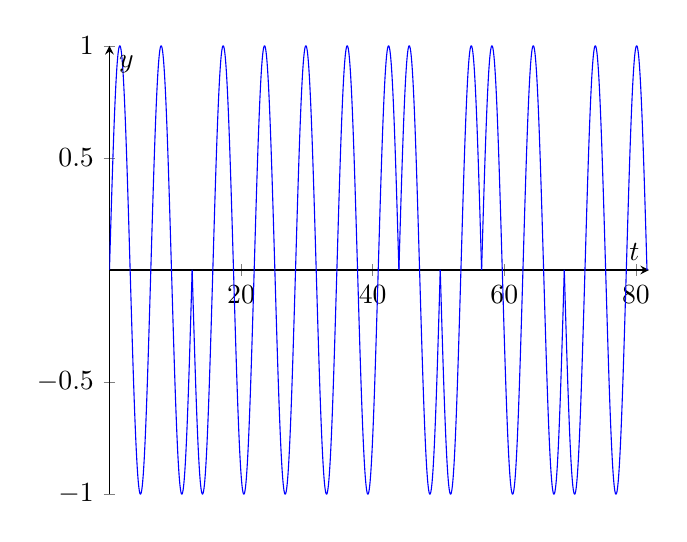
\begin{tikzpicture}
			\begin{axis}[
			xmin=0, xmax=82, xlabel=$t$,
			ymin=-1, ymax=1, ylabel=$y$,
			samples=400,
			axis x line=middle,
			axis y line=middle,
			domain=0:82,
			]
			\addplot[mark=none,smooth,blue,domain=0:2*pi] {sin(deg(x))};
			\addplot[mark=none,smooth,blue,domain=2*pi:4*pi] {sin(deg(x))};
			\addplot[mark=none,smooth,blue,domain=4*pi:6*pi] {sin(deg(x+pi))};
			\addplot[mark=none,smooth,blue,domain=6*pi:8*pi] {sin(deg(x+pi))};
			\addplot[mark=none,smooth,blue,domain=8*pi:10*pi] {sin(deg(x+pi))};
			\addplot[mark=none,smooth,blue,domain=10*pi:12*pi] {sin(deg(x+pi))};
			\addplot[mark=none,smooth,blue,domain=12*pi:14*pi] {sin(deg(x+pi))};
			\addplot[mark=none,smooth,blue,domain=14*pi:16*pi] {sin(deg(x))};
			\addplot[mark=none,smooth,blue,domain=16*pi:18*pi] {sin(deg(x+pi))};
			\addplot[mark=none,smooth,blue,domain=18*pi:20*pi] {sin(deg(x))};
			\addplot[mark=none,smooth,blue,domain=20*pi:22*pi] {sin(deg(x))};
			\addplot[mark=none,smooth,blue,domain=22*pi:24*pi] {sin(deg(x+pi))};
			\addplot[mark=none,smooth,blue,domain=24*pi:26*pi] {sin(deg(x+pi))};
			
			\end{axis}
			\end{tikzpicture}
		\end{center}
		\item Der Aufwand wächst vom Amplitudenverfahren zum Phasensprungverfahren, aber die Zuverlässigkeit der Verfahren auch.
	\end{enumerate}

	\section*{Aufgabe 4}
	\begin{enumerate}[label=(\alph*)]
		\item Anpassung des Datenstroms an das eingesetzte Übertragungsmedium
		\item Skizze:
		\begin{center}
			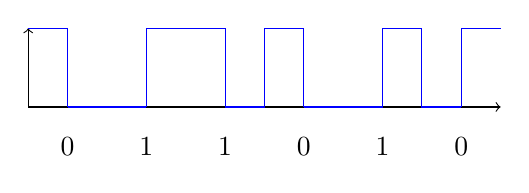
\begin{tikzpicture}
			\draw[->] (0,0) -- (6,0);
			\draw[->] (0,0) -- (0,1);
			
			\node at (0.5,-0.5) {0};
			\node at (1.5,-0.5) {1};
			\node at (2.5,-0.5) {1};
			\node at (3.5,-0.5) {0};
			\node at (4.5,-0.5) {1};
			\node at (5.5,-0.5) {0};
			
			\draw[blue] (0.5,0) -- (0.5,1);
			\draw[blue] (1.5,0) -- (1.5,1);
			\draw[blue] (2.5,0) -- (2.5,1);
			\draw[blue] (3.5,0) -- (3.5,1);
			\draw[blue] (4.5,0) -- (4.5,1);
			\draw[blue] (5.5,0) -- (5.5,1);
			
			\draw[blue] (0,1) -- (0.5,1);
			\draw[blue] (0.5,0) -- (1.5,0);
			\draw[blue] (1.5,1) -- (2.5,1);
			\draw[blue] (2.5,0) -- (3,0) -- (3,1) -- (3.5,1);
			\draw[blue] (3.5,0) -- (4.5,0);
			\draw[blue] (4.5,1) -- (5,1) -- (5,0) -- (5.5,0);
			\draw[blue] (5.5,1) -- (6,1);
			\end{tikzpicture}
		\end{center}
		\item Leitungscodes, Übertragungsrate = $\frac{1}{2}\cdot$ Signalrate
	\end{enumerate}

	\section*{Aufgabe 5}
	\begin{enumerate}[label=(\alph*)]
		\item durch feste Zeitschlitze (Taktung)
		\begin{itemize}
			\item synchrones Zeitmultiplex: Zuordnung zu virtuellem Kanal durch Position im Übertragungskanal
			\item asynchrones Zeitmultiplex: Channel Identifier für Zuordnung zu virtuellem Kanal
		\end{itemize}
		\item Das Frequenzband ist 223 MHz - 174 MHz = 49 MHz breit. Jeder Fernsehkanal braucht insgesamt 7 MHz (5.5 MHz für Daten + 1.5 MHz Sicherheitsabstand). Allerdings braucht der letzten Sender auf dem Frequenzband diesen Sicherheitsabstand nicht mehr. Insgesamt passen 7 Fernsehsender auf das Band, es bleiben 1.5 MHz übrig.
	\end{enumerate}
	
\end{document}